% Created by tikzDevice version 0.9 on 2016-02-03 14:00:42
% !TEX encoding = UTF-8 Unicode
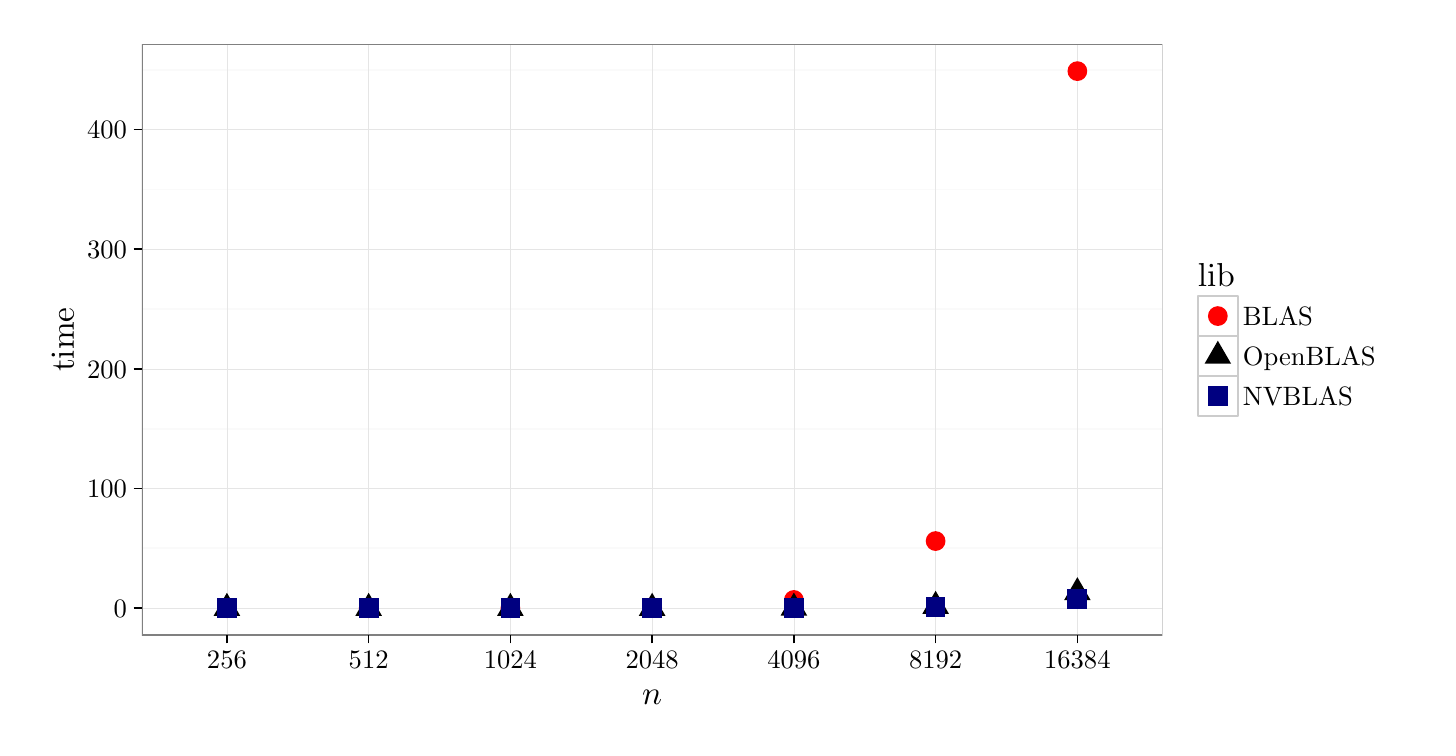
\begin{tikzpicture}[x=1pt,y=1pt]
\definecolor{fillColor}{RGB}{255,255,255}
\path[use as bounding box,fill=fillColor,fill opacity=0.00] (0,0) rectangle (505.89,252.94);
\begin{scope}
\path[clip] (  0.00,  0.00) rectangle (505.89,252.94);
\definecolor{drawColor}{RGB}{255,255,255}
\definecolor{fillColor}{RGB}{255,255,255}

\path[draw=drawColor,line width= 0.6pt,line join=round,line cap=round,fill=fillColor] ( -0.00,  0.00) rectangle (505.89,252.95);
\end{scope}
\begin{scope}
\path[clip] ( 41.26, 33.48) rectangle (410.03,246.94);
\definecolor{fillColor}{RGB}{255,255,255}

\path[fill=fillColor] ( 41.26, 33.48) rectangle (410.03,246.94);
\definecolor{drawColor}{gray}{0.98}

\path[draw=drawColor,line width= 0.6pt,line join=round] ( 41.26, 64.80) --
	(410.03, 64.80);

\path[draw=drawColor,line width= 0.6pt,line join=round] ( 41.26,108.03) --
	(410.03,108.03);

\path[draw=drawColor,line width= 0.6pt,line join=round] ( 41.26,151.27) --
	(410.03,151.27);

\path[draw=drawColor,line width= 0.6pt,line join=round] ( 41.26,194.50) --
	(410.03,194.50);

\path[draw=drawColor,line width= 0.6pt,line join=round] ( 41.26,237.74) --
	(410.03,237.74);
\definecolor{drawColor}{gray}{0.90}

\path[draw=drawColor,line width= 0.2pt,line join=round] ( 41.26, 43.18) --
	(410.03, 43.18);

\path[draw=drawColor,line width= 0.2pt,line join=round] ( 41.26, 86.41) --
	(410.03, 86.41);

\path[draw=drawColor,line width= 0.2pt,line join=round] ( 41.26,129.65) --
	(410.03,129.65);

\path[draw=drawColor,line width= 0.2pt,line join=round] ( 41.26,172.88) --
	(410.03,172.88);

\path[draw=drawColor,line width= 0.2pt,line join=round] ( 41.26,216.12) --
	(410.03,216.12);

\path[draw=drawColor,line width= 0.2pt,line join=round] ( 71.99, 33.48) --
	( 71.99,246.94);

\path[draw=drawColor,line width= 0.2pt,line join=round] (123.21, 33.48) --
	(123.21,246.94);

\path[draw=drawColor,line width= 0.2pt,line join=round] (174.43, 33.48) --
	(174.43,246.94);

\path[draw=drawColor,line width= 0.2pt,line join=round] (225.65, 33.48) --
	(225.65,246.94);

\path[draw=drawColor,line width= 0.2pt,line join=round] (276.87, 33.48) --
	(276.87,246.94);

\path[draw=drawColor,line width= 0.2pt,line join=round] (328.08, 33.48) --
	(328.08,246.94);

\path[draw=drawColor,line width= 0.2pt,line join=round] (379.30, 33.48) --
	(379.30,246.94);
\definecolor{fillColor}{RGB}{255,0,0}

\path[fill=fillColor] ( 71.99, 43.18) circle (  3.57);

\path[fill=fillColor] (123.21, 43.18) circle (  3.57);

\path[fill=fillColor] (174.43, 43.22) circle (  3.57);

\path[fill=fillColor] (225.65, 43.52) circle (  3.57);

\path[fill=fillColor] (276.87, 46.15) circle (  3.57);

\path[fill=fillColor] (328.08, 67.43) circle (  3.57);

\path[fill=fillColor] (379.30,237.24) circle (  3.57);
\definecolor{fillColor}{RGB}{0,0,0}

\path[fill=fillColor] ( 71.99, 48.74) --
	( 76.80, 40.41) --
	( 67.19, 40.41) --
	cycle;

\path[fill=fillColor] (123.21, 48.73) --
	(128.02, 40.41) --
	(118.40, 40.41) --
	cycle;

\path[fill=fillColor] (174.43, 48.73) --
	(179.23, 40.41) --
	(169.62, 40.41) --
	cycle;

\path[fill=fillColor] (225.65, 48.75) --
	(230.45, 40.43) --
	(220.84, 40.43) --
	cycle;

\path[fill=fillColor] (276.87, 48.83) --
	(281.67, 40.51) --
	(272.06, 40.51) --
	cycle;

\path[fill=fillColor] (328.08, 49.47) --
	(332.89, 41.14) --
	(323.28, 41.14) --
	cycle;

\path[fill=fillColor] (379.30, 54.39) --
	(384.11, 46.06) --
	(374.50, 46.06) --
	cycle;
\definecolor{fillColor}{RGB}{0,0,128}

\path[fill=fillColor] ( 68.42, 39.61) --
	( 75.56, 39.61) --
	( 75.56, 46.75) --
	( 68.42, 46.75) --
	cycle;

\path[fill=fillColor] (119.64, 39.61) --
	(126.78, 39.61) --
	(126.78, 46.75) --
	(119.64, 46.75) --
	cycle;

\path[fill=fillColor] (170.86, 39.61) --
	(178.00, 39.61) --
	(178.00, 46.75) --
	(170.86, 46.75) --
	cycle;

\path[fill=fillColor] (222.08, 39.62) --
	(229.22, 39.62) --
	(229.22, 46.76) --
	(222.08, 46.76) --
	cycle;

\path[fill=fillColor] (273.30, 39.68) --
	(280.43, 39.68) --
	(280.43, 46.82) --
	(273.30, 46.82) --
	cycle;

\path[fill=fillColor] (324.52, 40.08) --
	(331.65, 40.08) --
	(331.65, 47.21) --
	(324.52, 47.21) --
	cycle;

\path[fill=fillColor] (375.73, 43.05) --
	(382.87, 43.05) --
	(382.87, 50.18) --
	(375.73, 50.18) --
	cycle;
\definecolor{drawColor}{gray}{0.50}

\path[draw=drawColor,line width= 0.6pt,line join=round,line cap=round] ( 41.26, 33.48) rectangle (410.03,246.94);
\end{scope}
\begin{scope}
\path[clip] (  0.00,  0.00) rectangle (505.89,252.94);
\definecolor{drawColor}{RGB}{0,0,0}

\node[text=drawColor,anchor=base east,inner sep=0pt, outer sep=0pt, scale=  0.96] at ( 35.86, 39.87) {0};

\node[text=drawColor,anchor=base east,inner sep=0pt, outer sep=0pt, scale=  0.96] at ( 35.86, 83.11) {100};

\node[text=drawColor,anchor=base east,inner sep=0pt, outer sep=0pt, scale=  0.96] at ( 35.86,126.34) {200};

\node[text=drawColor,anchor=base east,inner sep=0pt, outer sep=0pt, scale=  0.96] at ( 35.86,169.58) {300};

\node[text=drawColor,anchor=base east,inner sep=0pt, outer sep=0pt, scale=  0.96] at ( 35.86,212.81) {400};
\end{scope}
\begin{scope}
\path[clip] (  0.00,  0.00) rectangle (505.89,252.94);
\definecolor{drawColor}{RGB}{0,0,0}

\path[draw=drawColor,line width= 0.6pt,line join=round] ( 38.26, 43.18) --
	( 41.26, 43.18);

\path[draw=drawColor,line width= 0.6pt,line join=round] ( 38.26, 86.41) --
	( 41.26, 86.41);

\path[draw=drawColor,line width= 0.6pt,line join=round] ( 38.26,129.65) --
	( 41.26,129.65);

\path[draw=drawColor,line width= 0.6pt,line join=round] ( 38.26,172.88) --
	( 41.26,172.88);

\path[draw=drawColor,line width= 0.6pt,line join=round] ( 38.26,216.12) --
	( 41.26,216.12);
\end{scope}
\begin{scope}
\path[clip] (  0.00,  0.00) rectangle (505.89,252.94);
\definecolor{drawColor}{RGB}{0,0,0}

\path[draw=drawColor,line width= 0.6pt,line join=round] ( 71.99, 30.48) --
	( 71.99, 33.48);

\path[draw=drawColor,line width= 0.6pt,line join=round] (123.21, 30.48) --
	(123.21, 33.48);

\path[draw=drawColor,line width= 0.6pt,line join=round] (174.43, 30.48) --
	(174.43, 33.48);

\path[draw=drawColor,line width= 0.6pt,line join=round] (225.65, 30.48) --
	(225.65, 33.48);

\path[draw=drawColor,line width= 0.6pt,line join=round] (276.87, 30.48) --
	(276.87, 33.48);

\path[draw=drawColor,line width= 0.6pt,line join=round] (328.08, 30.48) --
	(328.08, 33.48);

\path[draw=drawColor,line width= 0.6pt,line join=round] (379.30, 30.48) --
	(379.30, 33.48);
\end{scope}
\begin{scope}
\path[clip] (  0.00,  0.00) rectangle (505.89,252.94);
\definecolor{drawColor}{RGB}{0,0,0}

\node[text=drawColor,anchor=base,inner sep=0pt, outer sep=0pt, scale=  0.96] at ( 71.99, 21.46) {256};

\node[text=drawColor,anchor=base,inner sep=0pt, outer sep=0pt, scale=  0.96] at (123.21, 21.46) {512};

\node[text=drawColor,anchor=base,inner sep=0pt, outer sep=0pt, scale=  0.96] at (174.43, 21.46) {1024};

\node[text=drawColor,anchor=base,inner sep=0pt, outer sep=0pt, scale=  0.96] at (225.65, 21.46) {2048};

\node[text=drawColor,anchor=base,inner sep=0pt, outer sep=0pt, scale=  0.96] at (276.87, 21.46) {4096};

\node[text=drawColor,anchor=base,inner sep=0pt, outer sep=0pt, scale=  0.96] at (328.08, 21.46) {8192};

\node[text=drawColor,anchor=base,inner sep=0pt, outer sep=0pt, scale=  0.96] at (379.30, 21.46) {16384};
\end{scope}
\begin{scope}
\path[clip] (  0.00,  0.00) rectangle (505.89,252.94);
\definecolor{drawColor}{RGB}{0,0,0}

\node[text=drawColor,anchor=base,inner sep=0pt, outer sep=0pt, scale=  1.20] at (225.65,  8.40) {$n$};
\end{scope}
\begin{scope}
\path[clip] (  0.00,  0.00) rectangle (505.89,252.94);
\definecolor{drawColor}{RGB}{0,0,0}

\node[text=drawColor,rotate= 90.00,anchor=base,inner sep=0pt, outer sep=0pt, scale=  1.20] at ( 16.66,140.21) {time};
\end{scope}
\begin{scope}
\path[clip] (  0.00,  0.00) rectangle (505.89,252.94);
\definecolor{fillColor}{RGB}{255,255,255}

\path[fill=fillColor] (418.57,108.32) rectangle (491.35,172.10);
\end{scope}
\begin{scope}
\path[clip] (  0.00,  0.00) rectangle (505.89,252.94);
\definecolor{drawColor}{RGB}{0,0,0}

\node[text=drawColor,anchor=base west,inner sep=0pt, outer sep=0pt, scale=  1.20] at (422.84,159.57) {lib};
\end{scope}
\begin{scope}
\path[clip] (  0.00,  0.00) rectangle (505.89,252.94);
\definecolor{drawColor}{gray}{0.80}
\definecolor{fillColor}{RGB}{255,255,255}

\path[draw=drawColor,line width= 0.6pt,line join=round,line cap=round,fill=fillColor] (422.84,141.50) rectangle (437.29,155.95);
\end{scope}
\begin{scope}
\path[clip] (  0.00,  0.00) rectangle (505.89,252.94);
\definecolor{fillColor}{RGB}{255,0,0}

\path[fill=fillColor] (430.06,148.73) circle (  3.57);
\end{scope}
\begin{scope}
\path[clip] (  0.00,  0.00) rectangle (505.89,252.94);
\definecolor{drawColor}{gray}{0.80}
\definecolor{fillColor}{RGB}{255,255,255}

\path[draw=drawColor,line width= 0.6pt,line join=round,line cap=round,fill=fillColor] (422.84,127.04) rectangle (437.29,141.50);
\end{scope}
\begin{scope}
\path[clip] (  0.00,  0.00) rectangle (505.89,252.94);
\definecolor{fillColor}{RGB}{0,0,0}

\path[fill=fillColor] (430.06,139.82) --
	(434.87,131.50) --
	(425.26,131.50) --
	cycle;
\end{scope}
\begin{scope}
\path[clip] (  0.00,  0.00) rectangle (505.89,252.94);
\definecolor{drawColor}{gray}{0.80}
\definecolor{fillColor}{RGB}{255,255,255}

\path[draw=drawColor,line width= 0.6pt,line join=round,line cap=round,fill=fillColor] (422.84,112.59) rectangle (437.29,127.04);
\end{scope}
\begin{scope}
\path[clip] (  0.00,  0.00) rectangle (505.89,252.94);
\definecolor{fillColor}{RGB}{0,0,128}

\path[fill=fillColor] (426.50,116.25) --
	(433.63,116.25) --
	(433.63,123.39) --
	(426.50,123.39) --
	cycle;
\end{scope}
\begin{scope}
\path[clip] (  0.00,  0.00) rectangle (505.89,252.94);
\definecolor{drawColor}{RGB}{0,0,0}

\node[text=drawColor,anchor=base west,inner sep=0pt, outer sep=0pt, scale=  0.96] at (439.10,145.42) {BLAS};
\end{scope}
\begin{scope}
\path[clip] (  0.00,  0.00) rectangle (505.89,252.94);
\definecolor{drawColor}{RGB}{0,0,0}

\node[text=drawColor,anchor=base west,inner sep=0pt, outer sep=0pt, scale=  0.96] at (439.10,130.97) {OpenBLAS};
\end{scope}
\begin{scope}
\path[clip] (  0.00,  0.00) rectangle (505.89,252.94);
\definecolor{drawColor}{RGB}{0,0,0}

\node[text=drawColor,anchor=base west,inner sep=0pt, outer sep=0pt, scale=  0.96] at (439.10,116.51) {NVBLAS};
\end{scope}
\end{tikzpicture}
